\begin{figure}
\centering
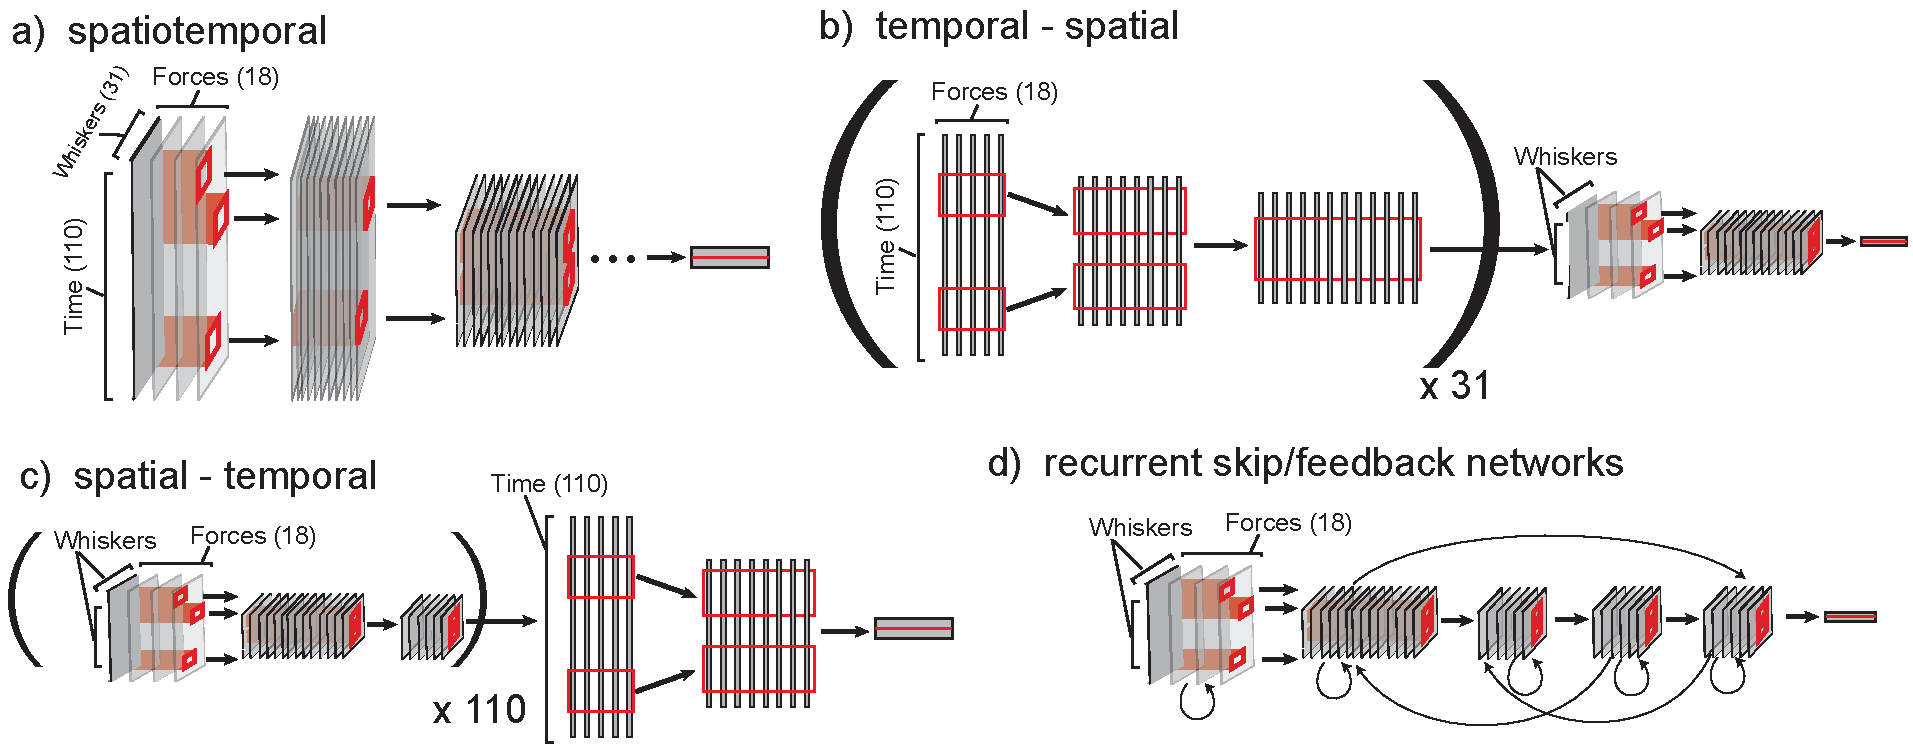
\includegraphics [width=1\linewidth]{figures/architectures.pdf}
\vspace{-2mm}
\caption{\textbf{Families of DNN Architectures tested:} \textbf{a.} Models with spatiotemporal integration at all stages. Convolution is performed on both spatial and temporal data dimensions, followed by one or several fully connected layers. \textbf{b.} Temporal-Spatial networks in which temporal integration is performed separately before spatial integration.  Temporal integration consists of one-dimensional convolution over the temporal dimension, separately for each whisker. the In spatial integration stages, outputs from each whisker are registered to their natural 2D spatial grid and spatial convolution performed.  \textbf{c.} In Spatial-Temporal networks, spatial convolution is performed first, replicated with shared weights across time points; this is then followed by temporal convolution. \textbf{d.} Recurrent networks with no explicitly separate units for handling for distinct timepoints, relying instead on state to build up memory traces.  These networks can have local recurrence (e.g. simple addition or more complicated motifs like LSTMs or GRUs), as well as long-range skip and feedback connections.~\label{fig_archi}}
\end{figure}

We trained deep neural networks of a variety of different architectural types on the shape-recognition task (Fig. \ref{fig_archi}).  
These architectures can be thought of as representing differing classes of hypotheses about the computations performed by neural circuits downstream of the whisker follicles. 
The fundamental questions explored by these hypotheses are how and where temporal and spatial information are integrated. 
Each architectural type is in fact a large family of related structures.  
Our strategy in identifying potential models of barrel cortex is to explore each family in terms of its ability to solve the shape recognition task in our training set, evaluating performance as well as efficiency (e.g. number of parameters and units needed). 


\subsubsection*{Simultaneous Spatiotemporal integration}

In this family of networks, networks consisted of convolution layers followed by one or more fully connected layers (Fig. \ref{fig_archi}a).  Convolution is performed on both temporal dimension and spatial dimensions of the input (and their corresponding downstream dimensions), so that that responses from nearby whiskers close in time are combined together simultaneously, with neurons in each successive layers having larger receptive field at both dimensions at once.
We evaluated both 2-dimensional convolution, in which the spatial dimension is indexed linearly across the list of whiskers (first by vertical columns and then by lateral row on the $5\times7$ grid), as well as 3-dimensional convolution in which the two dimensions of the $5\times7$ spatial grid are explicitly represented.
Data from top, middle, and bottom swipe of the same object combined to produce the final categorization, culminating in a standard softmax cross-entropy loss.  


\subsubsection*{Separate Spatial and Temporal Integration}

In this family, networks begin by integrating temporal and spatial information separately.  

One subclass of these networks are ``Temporal-Spatial'', which first integrate temporal information for each individual separately and then combine the information from different whiskers in higher layers (Fig. \ref{fig_archi}b).
Temporal processing is implemented as 1-dimensional convolution over the temporal dimension. 
After some number of layers of temporal-only processing, the outputs at each whisker are then reshaped into vectors and combined into a three-tensor in which the first two dimensions correspond to the $5\times7$ whisker grid spatial positions.  Subsequently, spatial convolutions are applied for some number of layers. 
Finally, as with previous case, features from three swipes  are concatenated into a single fully connected layer which produces softmax category responses.

Conversely, ``Spatial-Temporal'' networks (Fig. \ref{fig_archi}c) first, for some number of layers, use two-dimensional spatial convolution to integrate across whiskers, sharing parameters between copies of the network for each timepoint, before combining across time and switching to one-dimensional convolution in that dimension.  
Both Temporal-Spatial and Spatial-Temporal networks can be viewed as subclasses of three-dimensional simultaneous spatiotemporal integration in which initial and final portions of the network have kernel size 1 in the relevant dimensions.  
These network families can thus be thought of as different strategies for allocating parameters between dimensions. 


\subsubsection*{Recurrent neural networks}

This family of network does not allocate units or parameters explicitly for the temporal dimension, and instead requires temporal processing to occur via the temporal update evolution of the system.  These networks (Fig. \ref{fig_archi}d) are built around a core feedforward 2-dimensional spatial convolution structure, with the addition of (i) local recurrent connections, (ii) long-range feedforward skips between non-neighboring layers, and (iii) long-range feedback connections.  
Specifically, the update rule for the dynamic unrolling of such a network is: 

$$H^i_{t+1} = F_i \left ( \oplus_{j \neq i} R^j_t \right )  + \tau_i H^i_t; R^i_t = A_i[H^i_t]$$

where $R^i_t$ and $H^i_t$ are the output and hidden state of layer $i$ at time $t$ respectively,  $\tau_i$  are decay constants, $\oplus$ represents concatenation across the channel dimension with appropriate resizing to align dimensions, $F_i$ is the standard neural network update function (e.g. 2-D convolution), and $A_i$ is activation function at layer $i$.  The learned parameters of this network include the values of the parameters of $F_i$, which comprises both the feedforward and feedback weights from connections coming in to layer $i$, as well as the decay constants $\tau_i$. 



